\documentclass{article}

\usepackage[margin=0.5in]{geometry}
\usepackage{multicol}
\usepackage{graphicx}
\usepackage{siunitx}
\usepackage{amsthm}

\theoremstyle{definition}
\newtheorem*{solution}{Solution}

\title{Problem-Solving Set B}
\author{}
\date{}

\begin{document}
\maketitle
\begin{multicols}{2}
    \begin{enumerate}
        \item What is the degree measure of angle $A$?
            \begin{center}
                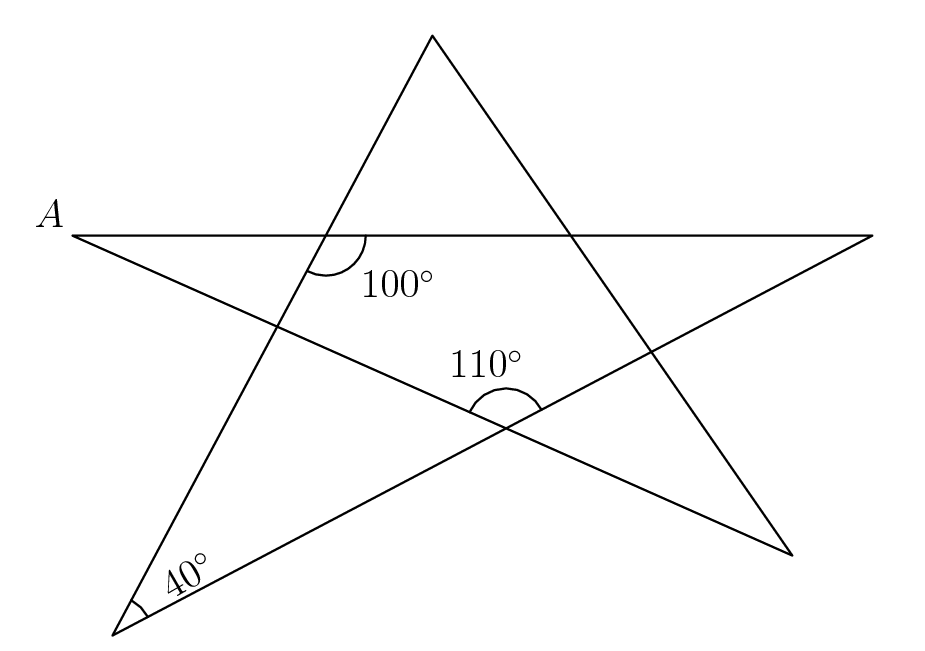
\includegraphics[scale=0.15]{star.png}
            \end{center}
            \begin{solution}
                The third angle of the triangle containing the $\ang{100}$ angle and the $\ang{40}$ is $\ang{180} - \ang{100} - \ang{40} = \ang{40}$.
                If follows that $A$ is the third angle of the triangle consisting of the found $\ang{40}$ angle and the given $\ang{110}$ angle.
                Thus, $A$ is a $\ang{180} - \ang{110} - \ang{40} = \ang{30}$ angle.
            \end{solution}
        \item What is the remainder of $1999^{2000}$ when it is divided by $5$?
            \begin{solution}
                Note that the units digits of the powers of $9$ have a pattern: $9^1 = 9$, $9^2 = 81$, $9^3 = 729$, $9^ = 6561$, and so on.
                Since all natural numbers with the same last digit have the same remainder when divided by $5$, the entire number doesn't matter, just the last digit.
                For even powers of $9$, the number ends in a $1$.
                Since the exponent is even, the final digit is $1$.
                Note that all natural numbers that end in $1$ have a remainder of $1$ when divided by $5$.
                So, our answer is $1$.
            \end{solution}
        \item Harold tosses a nickel four times.
            What is the probability that he gets at least as many heads as tails?
            \begin{solution}
                \textbf{Case 1:} There are two heads, two tails.
                The number of ways to choose which two tosses are heads is ${4}\choose{2} = 6$, and the other two must be tails. \\
                \textbf{Case 2:} There are three heads, one tail.
                There are ${4}\choose{1} = 4$ ways to choose which of the four tosses is a tail. \\
                \textbf{Case 3:} There are four heads, no tails.
                This can only happen $1$ way. \\
                There are a total of $2^4 = 16$ possible configurations, giving a probability of $\frac{6 + 4 + 1}{16} = \frac{11}{16}$.
            \end{solution}
        \item Loki, Moe, Nick, and Ott are good friends.
            Ott had no money, but the others did.
            Moe gave Ott one-fifth of his money, Loki gave Ott one-fourth of his money, and Nick gave Ott one-third of his money.
            Each gave Ott the same amount of money.
            What fractional part of the group's money does Ott have now?
            \begin{solution}
                Since Ott gets equal amounts of money from each friend, we can say that the gets $x$ dollars from each friend.
                This means that Moe has $5x$ dollars, Loki has $4x$ dollars, and Nick has $3x$ dollars.
                The total amount is $12x$ dollars, and since Ott gets $3x$ dollars total, $\frac{3x}{12x} = \frac{3}{12} = \frac{1}{4}$.
            \end{solution}
        \item Bicycle license plats in Flatville each contain three letters.
            The first is chosen from the set $\{C,H,L,P,R\}$, the second from $\{A,I,O\}$, and the third from $\{D,M,N,T\}$.
            When Flatville needed more license plates, they added two new letters, The new letters may both be added to one set or one letter may be added to one set and one to another set.
            What is the largest possible number of ADDITIONAL license plates that can be made by adding two letters?
            \begin{solution}
                Before new letters were added, five different letters could have been chosen for the first position, three for the second, and four for the third.
                This means that $5 \cdot 3 \cdot 4 = 60$ plates could have been made. \\
                If two letters are added to the second set, then $5 \cdot 5 \cdot 4 = 100$ plates can be made.
                If one letter is added to each of the second and third sets, then $5 \cdot 4 \cdot 5 = 100$ plates can be made.
                None of the other four ways to place the two letters will create as many plates.
                So, $100 - 60 = 40$ ADDITIONAL plates can be made.
            \end{solution}
    \end{enumerate}
\end{multicols}
\end{document}